\documentclass[12pt,pdf,hyperref={unicode}]{beamer}


%\documentclass[10pt]{beamer}

\usetheme[progressbar=frametitle]{metropolis}

\usepackage{booktabs}
\usepackage[scale=2]{ccicons}

\usepackage{pgfplots}
\usepgfplotslibrary{dateplot}

\usepackage{xspace}
\newcommand{\themename}{\textbf{\textsc{metropolis}}\xspace}


%\usepackage{lmodern}

% подключаем кириллицу 
\usepackage[T2A]{fontenc}
\usepackage[utf8]{inputenc}
\usepackage{listings}
%\usepackage{graphicx}
\usepackage{hyperref}

% отключить клавиши навигации
\setbeamertemplate{navigation symbols}{}

% тема оформления
\usetheme{Pittsburgh}

% цветовая схема
\usecolortheme{default}

\definecolor{light-gray}{gray}{0.90}

\title{Семинар №11}   
\subtitle{ФАКИ \the\year}
\author{Бирюков В. А.} 
\date{\today}
% \logo{
\includegraphics[height=5mm]{images/logo.png}\vspace{-7pt}}

\begin{document}

\lstset{language=C}

% титульный слайд
\begin{frame}
\titlepage
\end{frame} 



\defverbatim[colored]\makeset{
\begin{lstlisting}[language=C++,basicstyle=\ttfamily,keywordstyle=\color{blue},
                stringstyle=\color{red}\ttfamily]
void make_set(int X) {
  parent[X] = X;
}
\end{lstlisting}
}

\lstset{
  language=C,                % choose the language of the code
  keywordstyle=\color{blue},
  numbers=none,                   % where to put the line-numbers
  stepnumber=1,                   % the step between two line-numbers.        
  numbersep=5pt,                  % how far the line-numbers are from the code
  backgroundcolor=\color{light-gray},  % choose the background color. You must add \usepackage{color}
  showspaces=false,               % show spaces adding particular underscores
  showstringspaces=false,         % underline spaces within strings
  showtabs=false,                 % show tabs within strings adding particular underscores
  tabsize=2,                      % sets default tabsize to 2 spaces
  captionpos=b,                   % sets the caption-position to bottom
  breaklines=true,                % sets automatic line breaking
  breakatwhitespace=true,         % sets if automatic breaks should only happen at whitespace
}




\section{Структуры данных}


\begin{frame}[fragile]
\frametitle{Структуры данных}
\begin{itemize}
\item Структура данных (англ. data structure) — определённый способ организации данных, так, чтобы их можно было использовать эффективно.
\item Для разных задач более эффективными будут разные структуры данных.
\end{itemize}
\end{frame}

\begin{frame}[fragile]
\frametitle{Массив}
\begin{itemize}
\item Простейшая структура данных \\
\item Статический или динамический \\
\item Базовые операции:
\begin{enumerate}
\item index  --  доступ к элементу
\item insert --  добавить элемент
\item remove --  удалить элемент
\item find   --  найти элемент
\end{enumerate}
\end{itemize}
\end{frame}


\begin{frame}[fragile]
\frametitle{Массив}
\begin{center}
  \begin{tabular}{  l | c }
      & Массив \\
    \hline
    index & O(1) \\
    insert & O(1)  \\
    remove & O(N) \\
    find & O(N)  \\
    \hline
  \end{tabular}
\end{center}
\end{frame}


\begin{frame}[fragile]
\frametitle{Упорядоченный массив}
\framesubtitle{Бинарный поиск} 
\begin{center}
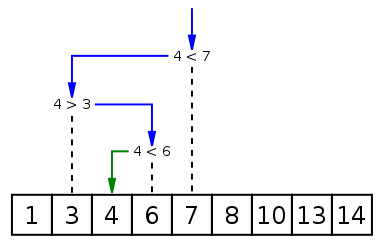
\includegraphics[width=0.7\linewidth]{images/Binary_search_into_array.png}
\end{center}
\end{frame}


\begin{frame}[fragile]
\frametitle{Упорядоченный массив}
\begin{center}
  \begin{tabular}{  l | c r }
      & Массив & Упорядоченный массив \\
    \hline
    index & O(1) & O(1)\\
    insert & O(1) & O(N)\\
    remove & O(N) & O(N)\\
    find & O(N) & O($\log(N)$)\\
    \hline
  \end{tabular}
\end{center}
\end{frame}


\section{Связный список}

\begin{frame}[fragile]
\frametitle{Связный список} 
\begin{lstlisting}[language=C++,basicstyle=\ttfamily,keywordstyle=\color{blue},stringstyle=\color{orange}\ttfamily]
struct Node {
	int data;
	struct Node * next;
};
struct Node * head;
\end{lstlisting}
\end{frame}




\begin{frame}[fragile]
\frametitle{Связный список} 
\begin{center}
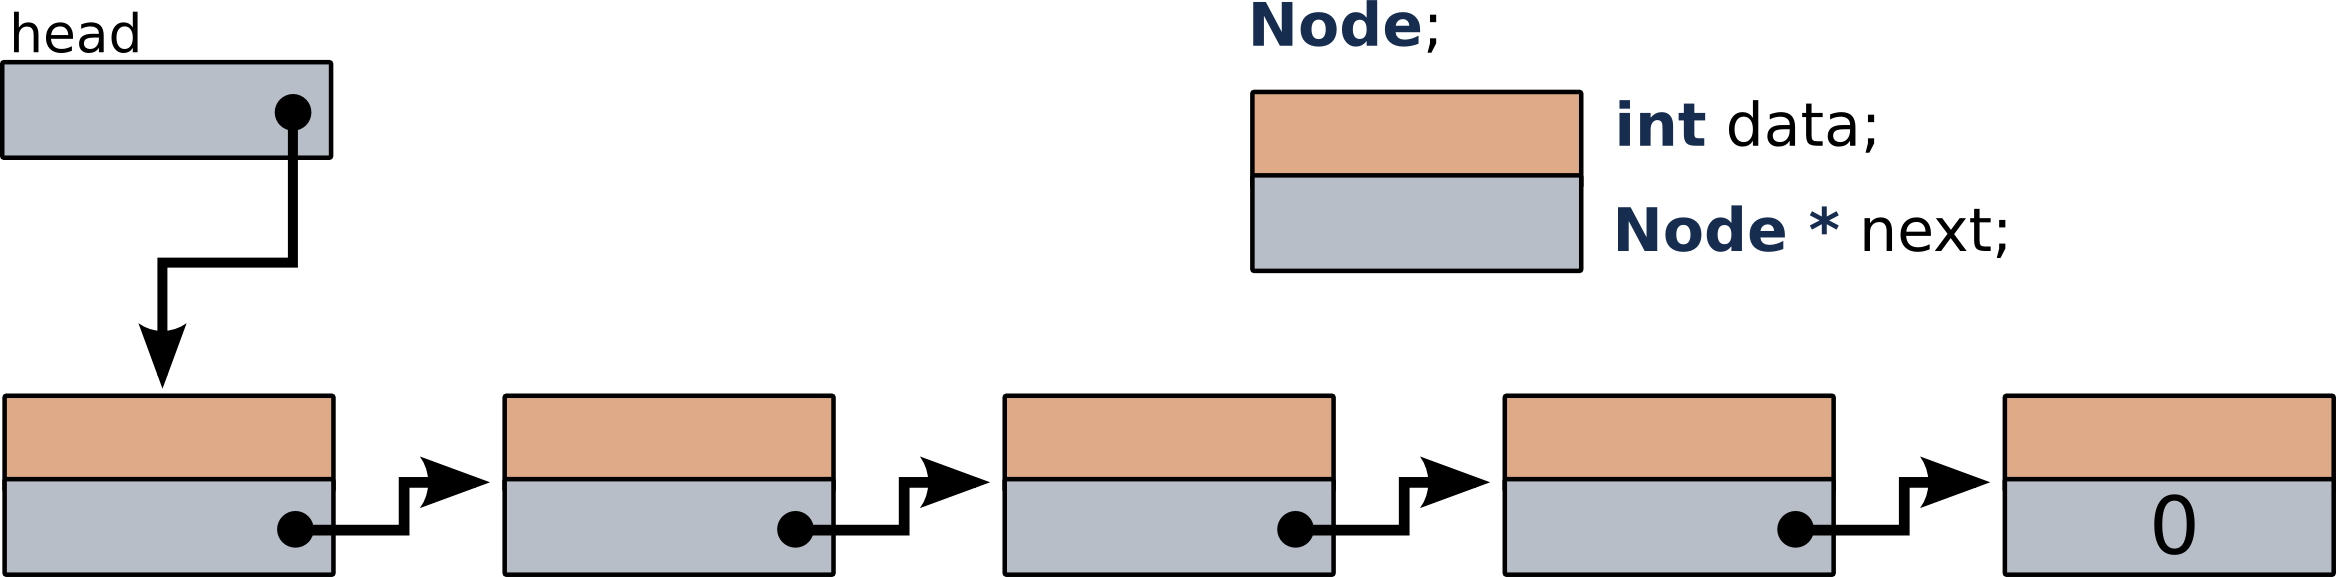
\includegraphics[width=0.99\linewidth]{images/list_initial.png}
\end{center}
\end{frame}


\begin{frame}[fragile]
\frametitle{Связный список} 
\framesubtitle{Обход связного списка - 1} 
\begin{center}
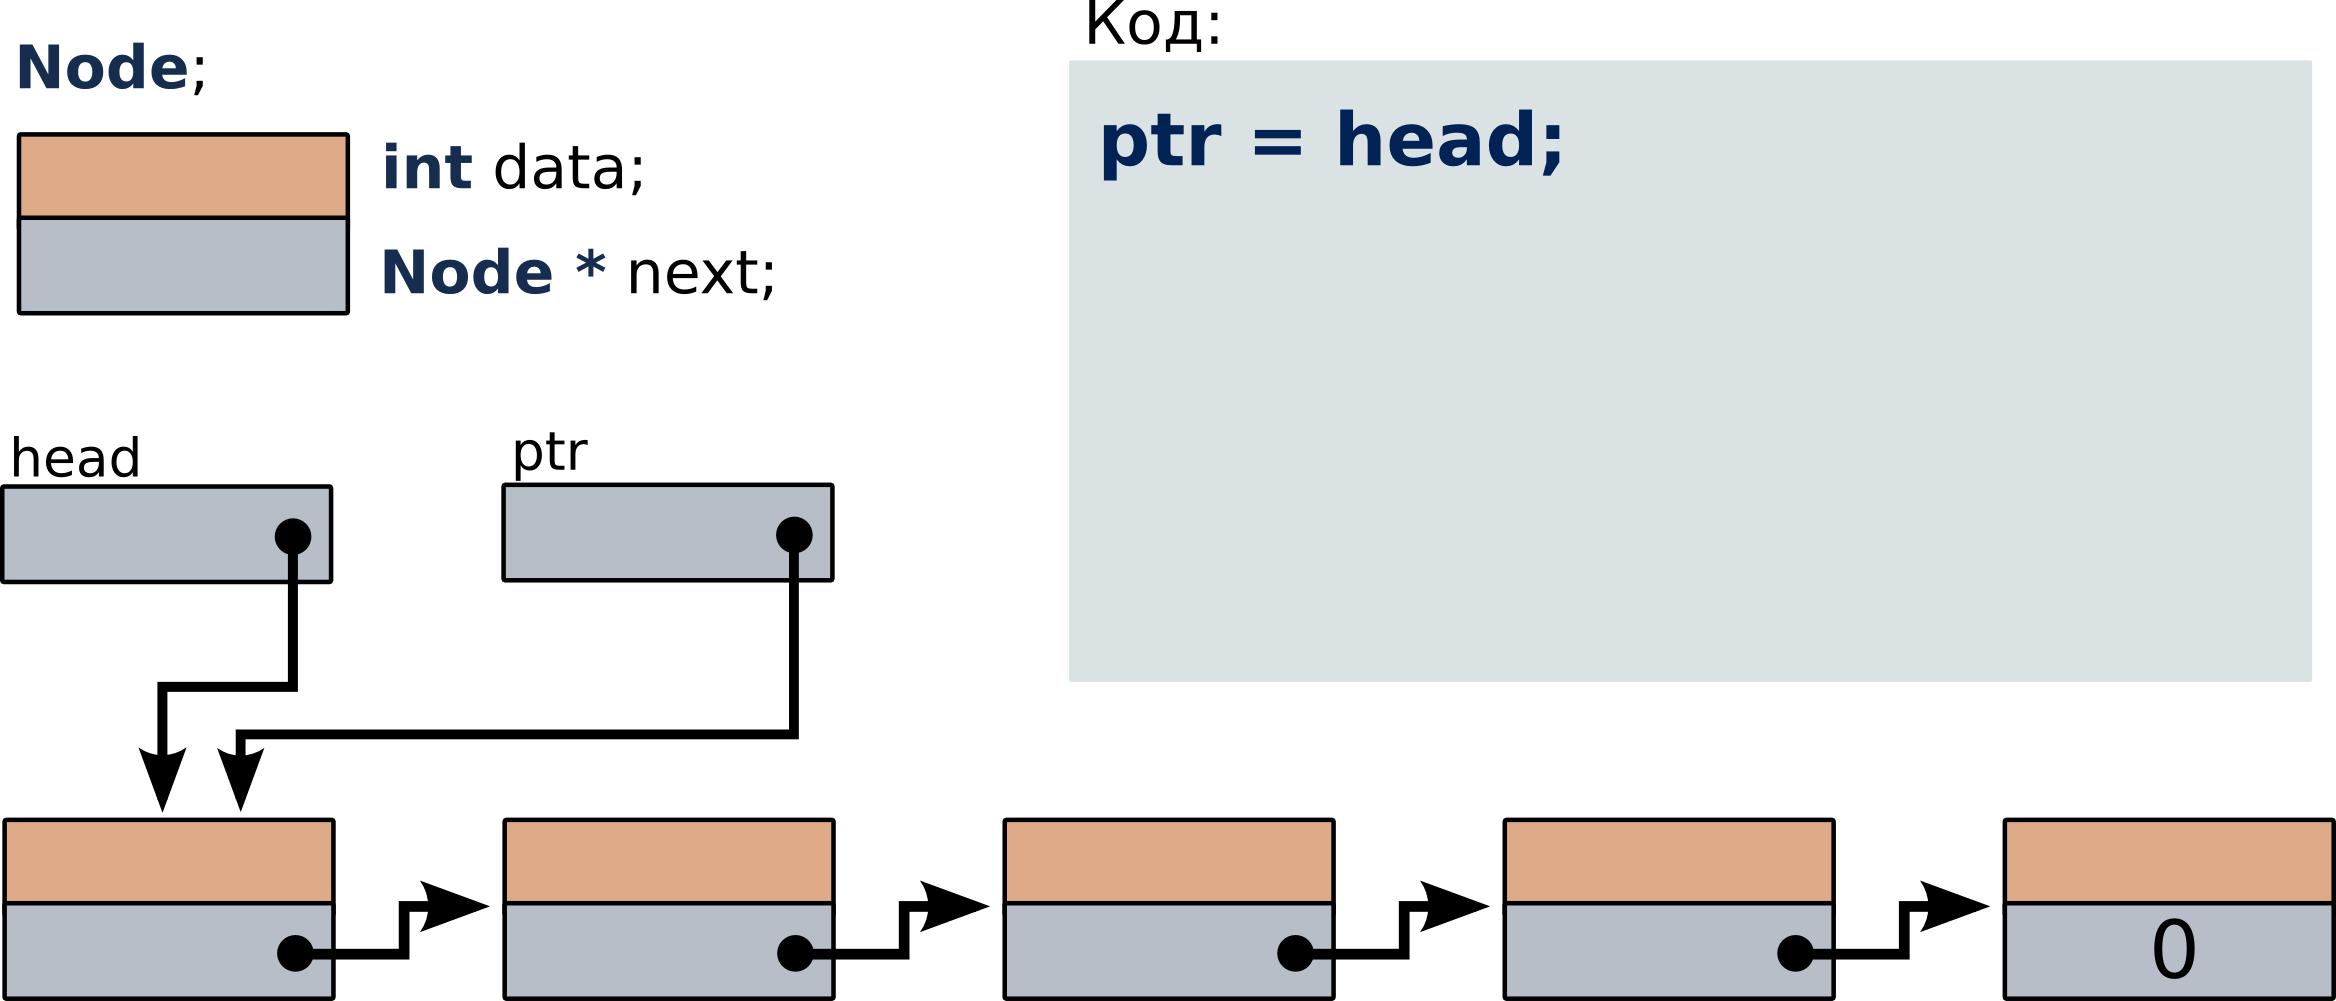
\includegraphics[width=0.99\linewidth]{images/list_traversal_1.png}
\end{center}
\end{frame}
\begin{frame}[fragile]
\frametitle{Связный список} 
\framesubtitle{Обход связного списка - 2} 
\begin{center}
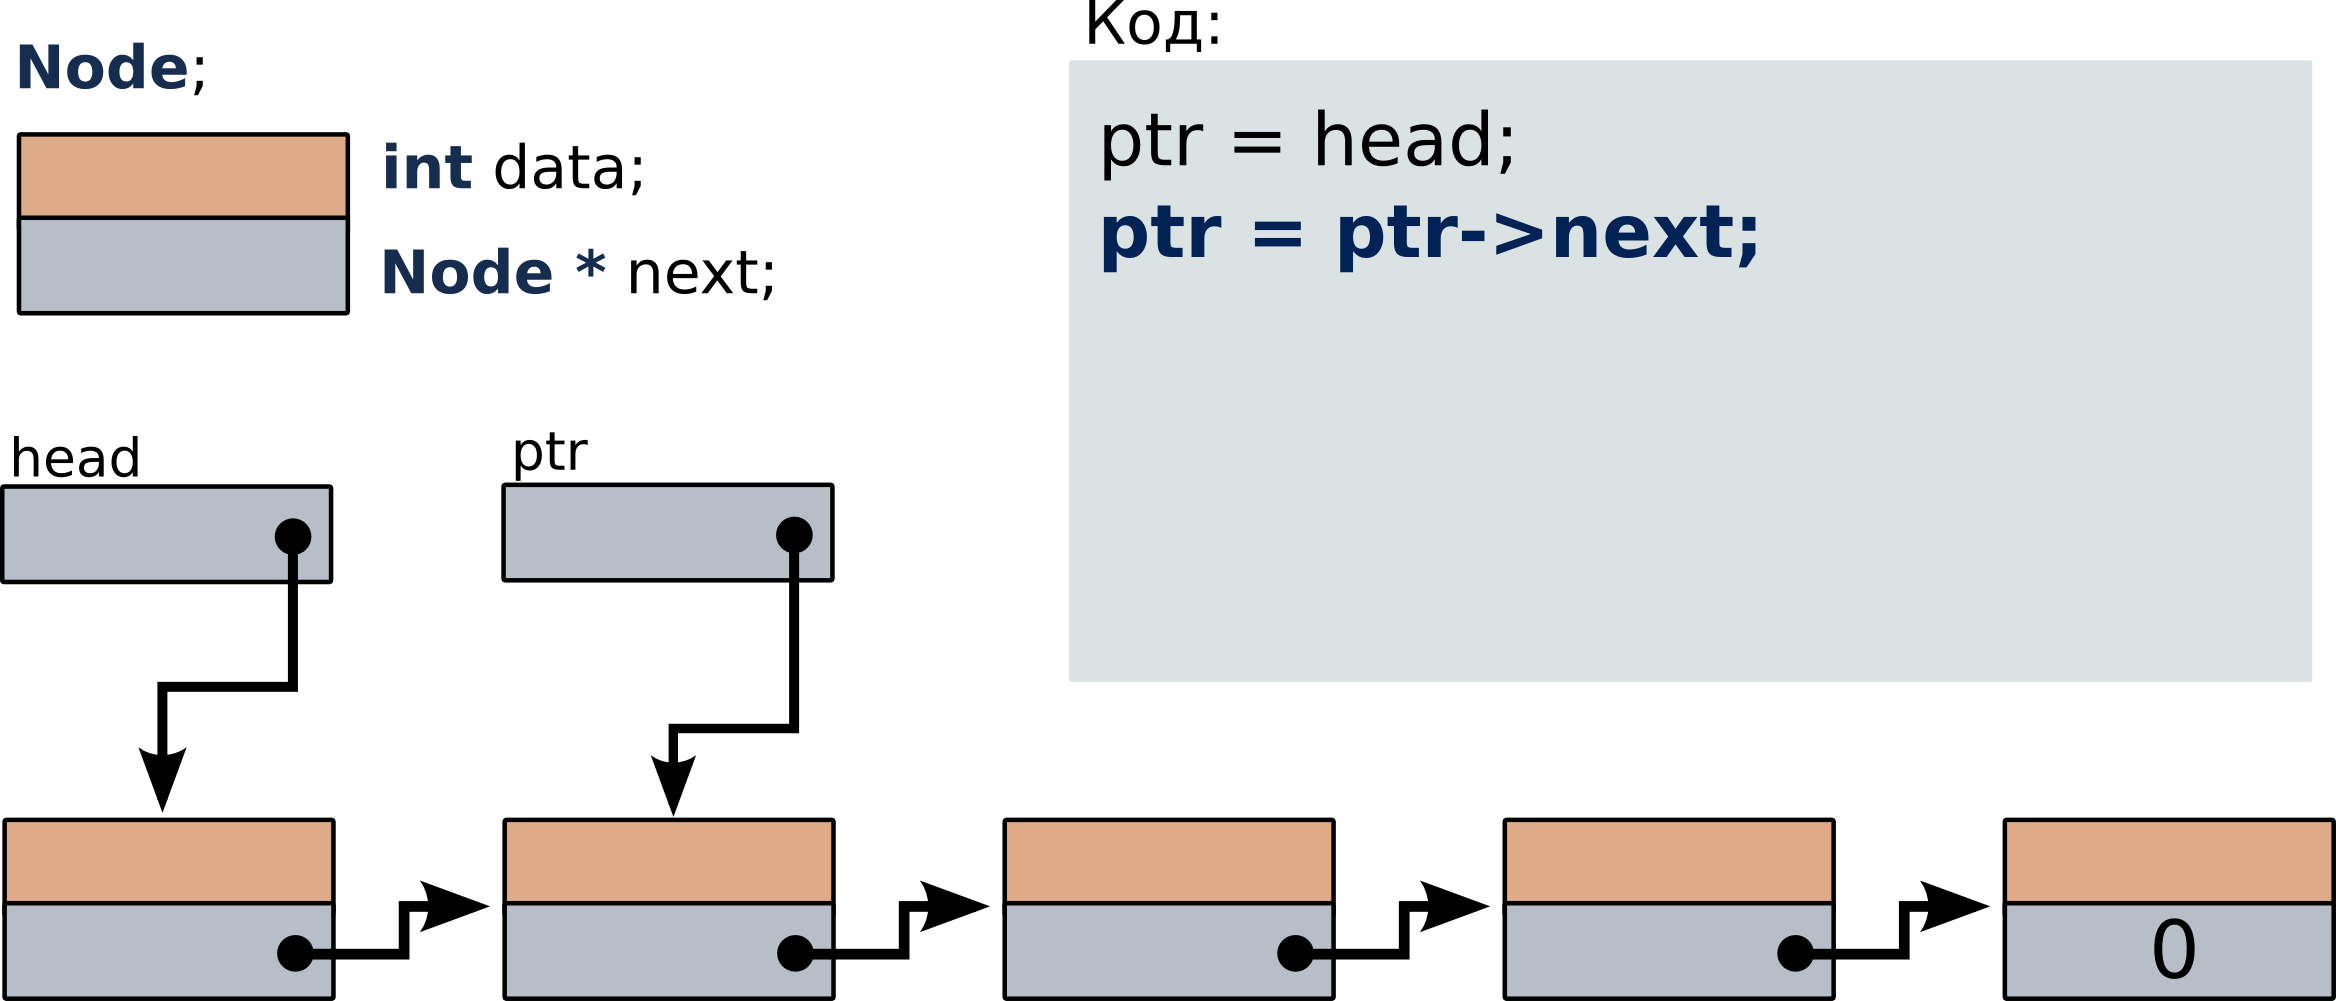
\includegraphics[width=0.99\linewidth]{images/list_traversal_2.png}
\end{center}
\end{frame}
\begin{frame}[fragile]
\frametitle{Связный список} 
\framesubtitle{Обход связного списка - 3} 
\begin{center}
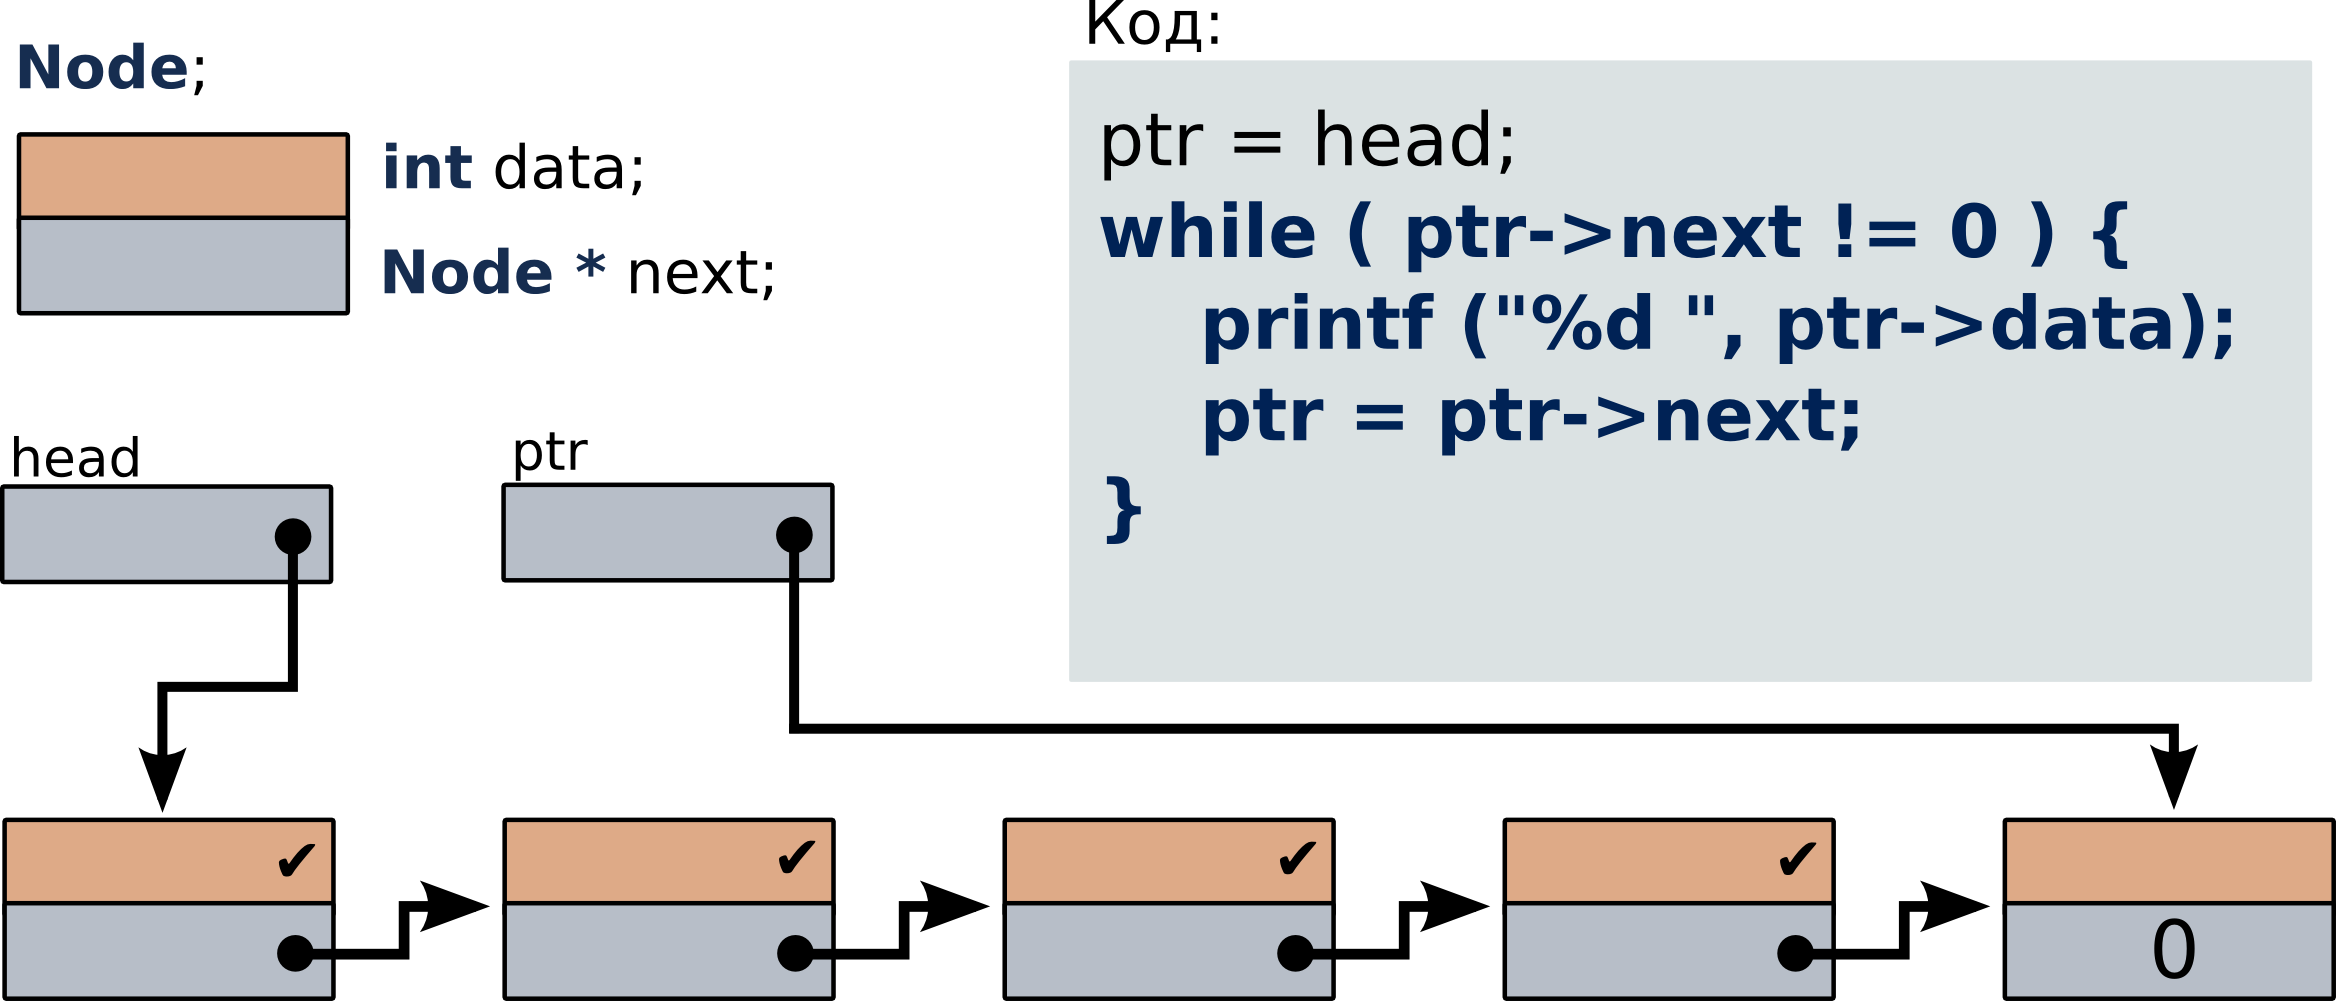
\includegraphics[width=0.99\linewidth]{images/list_traversal_3.png}
\end{center}
\end{frame}

\begin{frame}[fragile]
\frametitle{Связный список} 
\framesubtitle{Удаление элемента списка - 1} 
\begin{center}
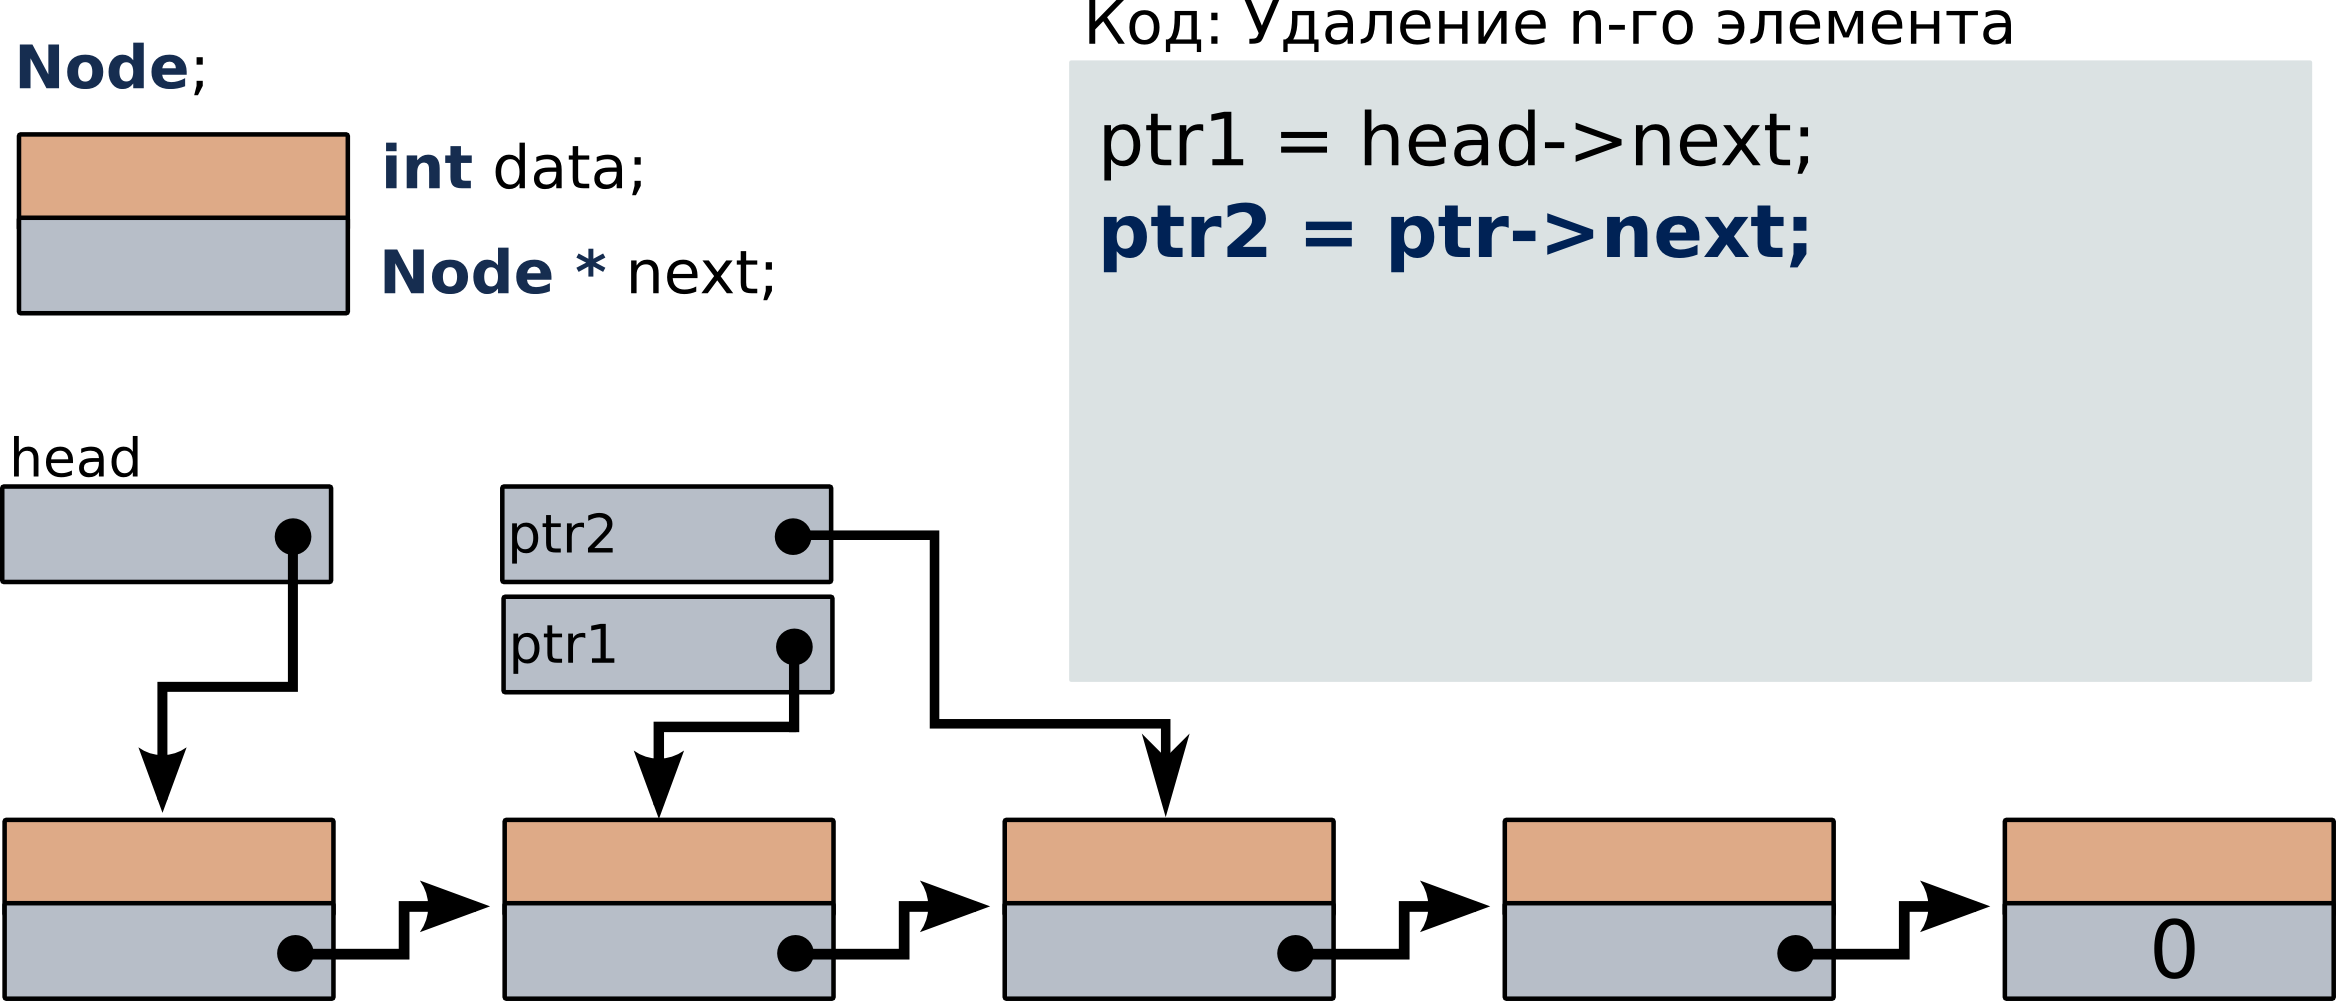
\includegraphics[width=0.99\linewidth]{images/list_delete_1.png}
\end{center}
\end{frame}
\begin{frame}[fragile]
\frametitle{Связный список} 
\framesubtitle{Удаление элемента списка - 2} 
\begin{center}
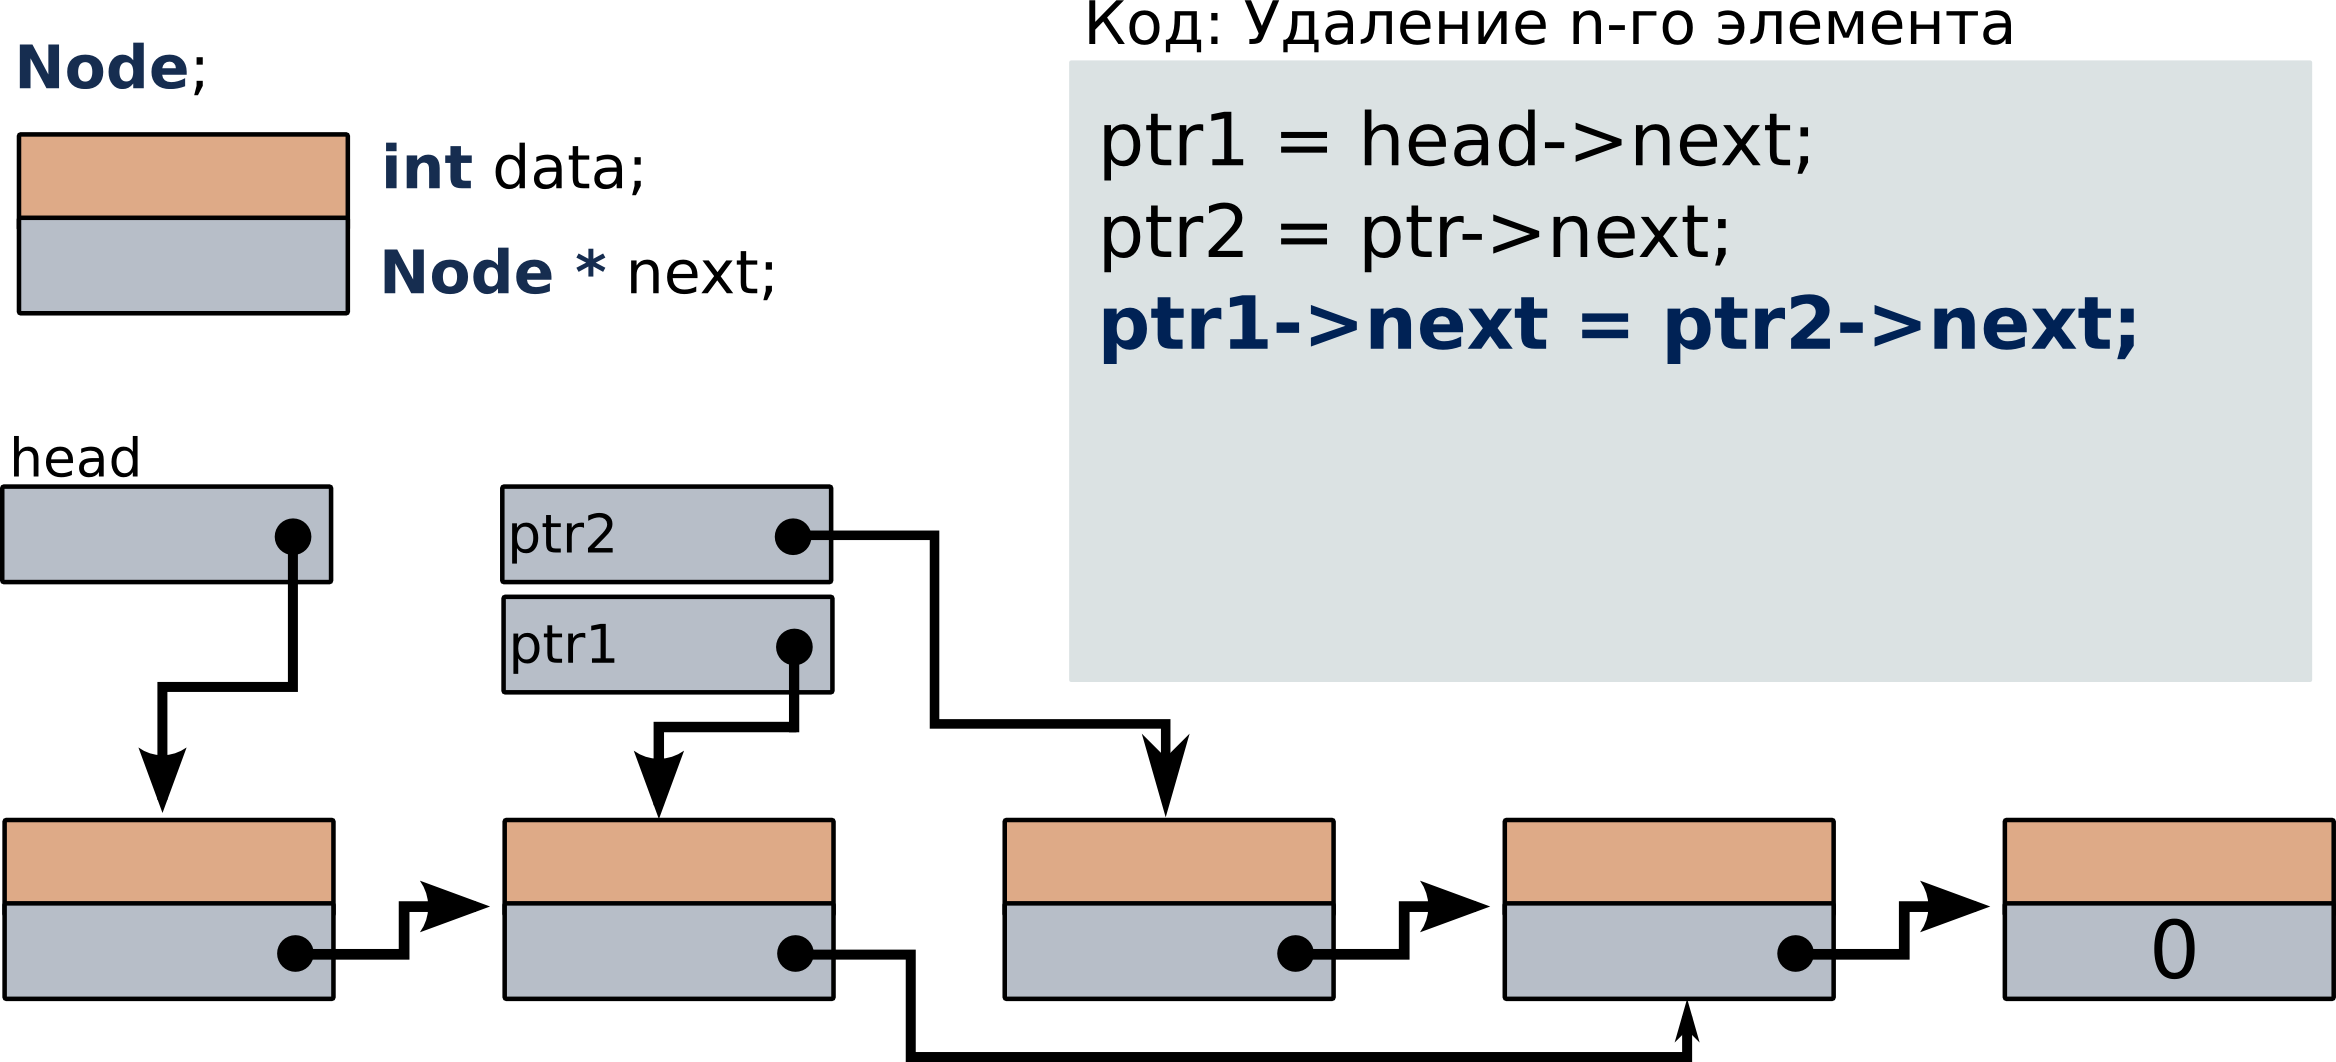
\includegraphics[width=0.99\linewidth]{images/list_delete_2.png}
\end{center}
\end{frame}
\begin{frame}[fragile]
\frametitle{Связный список} 
\framesubtitle{Удаление элемента списка - 3} 
\begin{center}
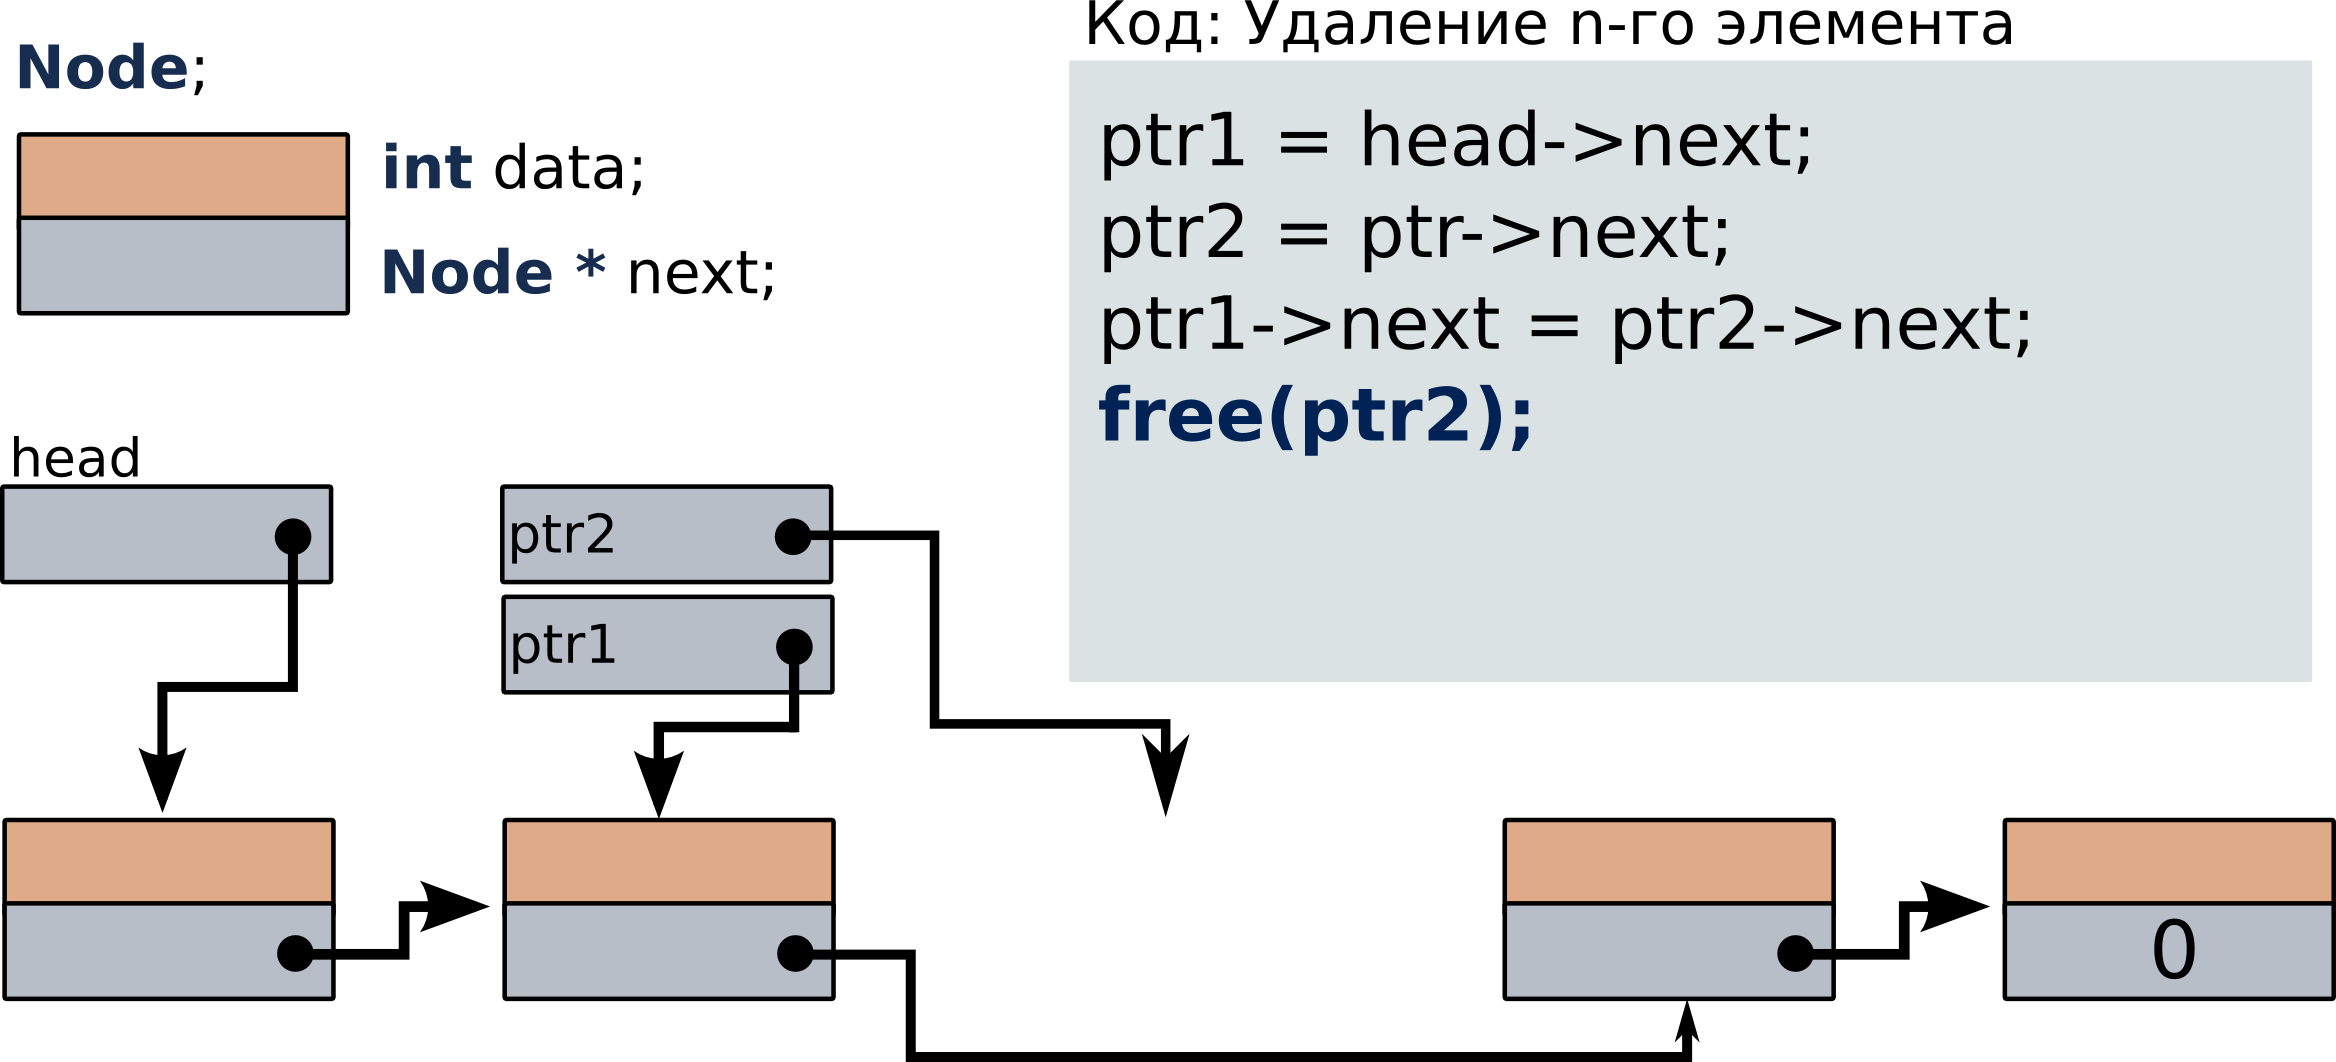
\includegraphics[width=0.99\linewidth]{images/list_delete_3.png}
\end{center}
\end{frame}



\begin{frame}[fragile]
\frametitle{Связный список}
\begin{itemize}
\item Простейшая структура данных \\
\item Динамический \\
\item Базовые операции:
\begin{enumerate}
\item index  --  доступ к элементу
\item insertToFront --  добавить элемент в начало
\item insertToBack --  добавить элемент в конец
\item insertAfter  --  добавить элемент после данного
\item insertBefore  --  добавить элемент перед данным
\item remove --  удалить Известный элемент
\item find   --  найти элемент
\end{enumerate}
\end{itemize}
\end{frame}


\begin{frame}[fragile]
\frametitle{Связный список}
\begin{center}
  \begin{tabular}{  l | c }
      & Список \\
    \hline
    index & O(N) \\
    insertToFront & O(1)  \\
    insertToBack & O(N)  \\
    insertAfter & O(1)  \\
    insertBefore & O(N)  \\
    remove & O(1) \\
    find & O(N)  \\
    \hline
  \end{tabular}
\end{center}
\end{frame}


\begin{frame}[fragile]
\frametitle{Двусвязный список} 
\begin{center}
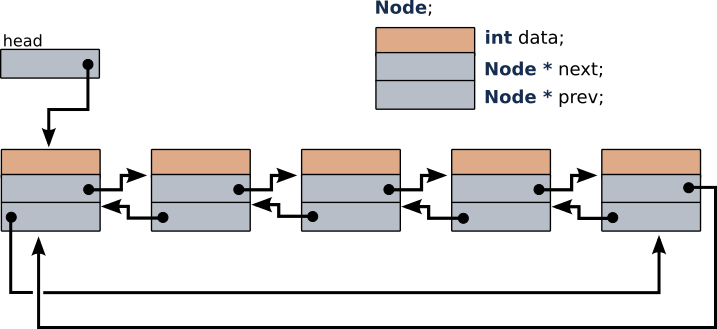
\includegraphics[width=0.99\linewidth]{images/2linked_list.png}
\end{center}
\end{frame}


\begin{frame}[fragile]
\frametitle{Двусвязный список}
\begin{center}
  \begin{tabular}{  l | c r }
      & Список & Двусвязный список \\
    \hline
    index & O(N) &  O(N) \\
    insertToFront & O(1) & O(1) \\
    insertToBack & O(N) & O(1) \\
    insertAfter & O(1) & O(1) \\
    insertBefore & O(N) & O(1) \\
    remove & O(1) & O(1) \\
    find & O(N) & O(N) \\
    \hline
  \end{tabular}
\end{center}
\end{frame}



\section{Valgrind}




\section{Задание}

\begin{frame}[fragile]
\frametitle{Задание} 
\begin{itemize}
\item Контест на списки
\end{itemize}
\end{frame}

\end{document}
